\documentclass[a4paper, portrait,11pt]{article}
\usepackage{polski}
\usepackage[utf8]{inputenc}
\usepackage{amsmath}
\usepackage{graphicx}
\usepackage{hyperref}
\usepackage{listings}
\usepackage{subcaption}
\usepackage{numprint}
\usepackage{siunitx}
\usepackage[justification=centering]{caption}
\usepackage[margin=0.5in]{geometry}
\npdecimalsign{.}
\nprounddigits{3}

\title{\textbf{Zadanie 3 - Inteligentna Analiza Danych}}
\author{
  Adam Zambrzycki\\
  \texttt{Nr indeksu: 216933}
  \and
  Konrad Stępniak\\
  \texttt{Nr indeksu: 216892}
}

\begin{document}
\maketitle
  \begin{tabular}{ll}
    \textbf{Kierunek} & Informatyka\\
    \textbf{Rok akademicki} & {2018/19} \\
    \textbf{Semestr} & {4} \\
    \textbf{Grupa dziekańska}& {2} \\ \\ \\
  \end{tabular}

Symbol $\alpha$ będzie oznaczał współczynnik nauki, a $K$ liczbę centrów.
Współczynnik skalujący w sieci będzie nazywany sigmą.

\section{Osobna nauka warstw - Aproksymacja}
Do nauki wykorzystano następujące parametry: $\alpha=0.05$, liczba iteracji $= 20000$.
Optymalną sigmę uzyskano ze wzoru:
\begin{equation}
  \sigma = \frac{d}{\sqrt{2M}}
\end{equation}
Gdzie $d$ - maksymalna odległość między centrami, a $M$ to liczba centrów.
\subsection{Podzadanie 1}

\begin{figure}[!htb]
  \begin{minipage}{0.33\textwidth}
    \centering
    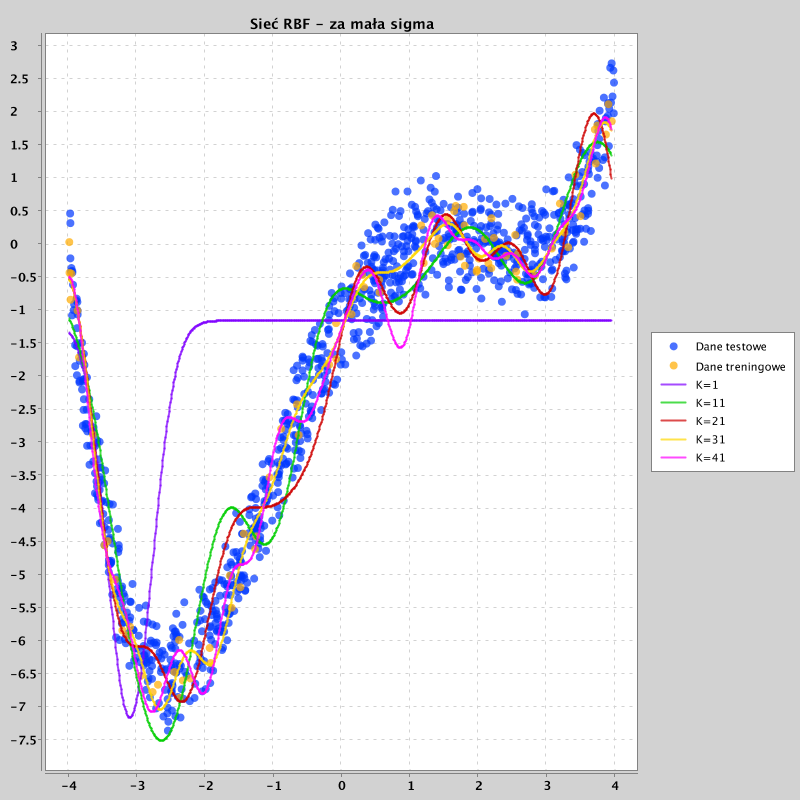
\includegraphics[width=1\linewidth]{../data/approximation3/1/small.png}
    \caption{\label{fig:1small}Za mała sigma}
  \end{minipage}
  \begin{minipage}{0.33\textwidth}
    \centering
    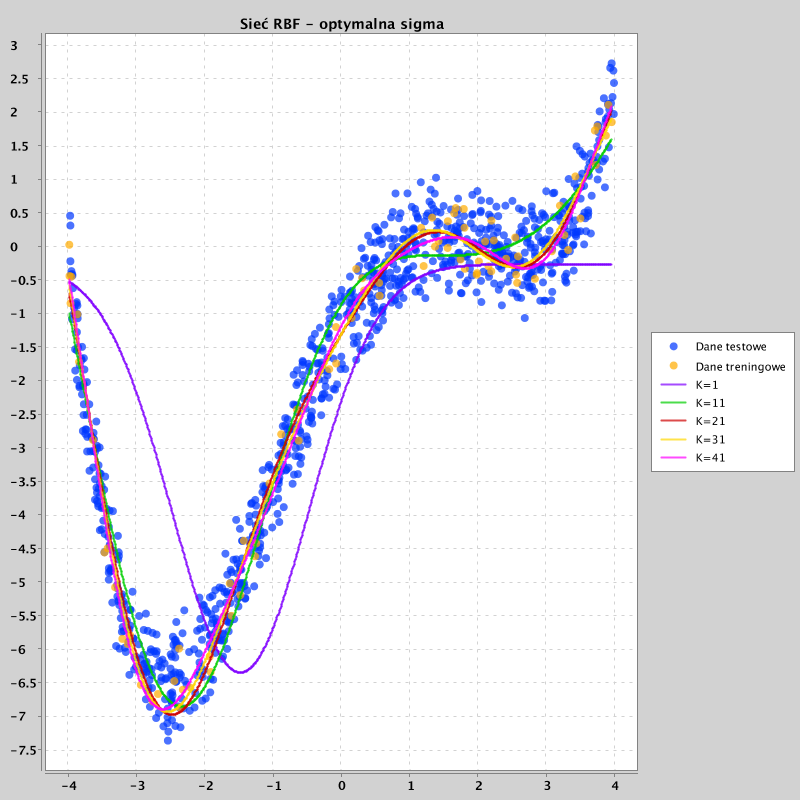
\includegraphics[width=1\linewidth]{../data/approximation3/1/optimal.png}
    \caption{\label{fig:1optimal}Optymalna sigma}
  \end{minipage}
  \begin{minipage}{0.33\textwidth}
    \centering
    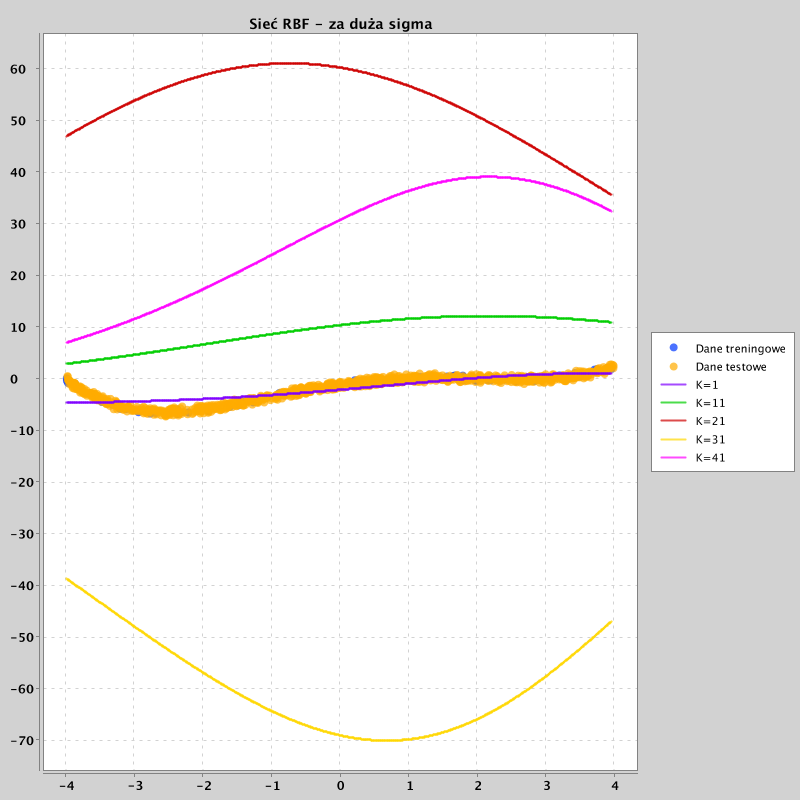
\includegraphics[width=1\linewidth]{../data/approximation3/1/big.png}
    \caption{\label{fig:1big}Za duża sigma}
  \end{minipage}\hfill
\end{figure}
Dla liczby $K >= 11$, gdy współczynnik skalujący 
jest zbyt mały sieć przybliża dane treningowe do pewnego stopnia, 
jednak tworzy pewne zakłócenia, co daje niedokładne przybliżenie.
Z drugiej strony, gdy sigma jest zbyt duża sieć praktycznie wcale nie aproksymuje danych jedynie je przecina w pewien sposób.
Sieć o $K=1$ daje takie same wyniki, jak $K=41$.
Gdy sigma jest optymalna, sieć o każdej liczbie neuronów oprócz $K=1$, aproksymuje tak samo dokładnie.

\subsection{Podzadanie 2}

Czerwone linie reprezentują funkcje pojedynczych neuronów.
\begin{figure}[!htb]
  \begin{minipage}{0.33\textwidth}
    \centering
    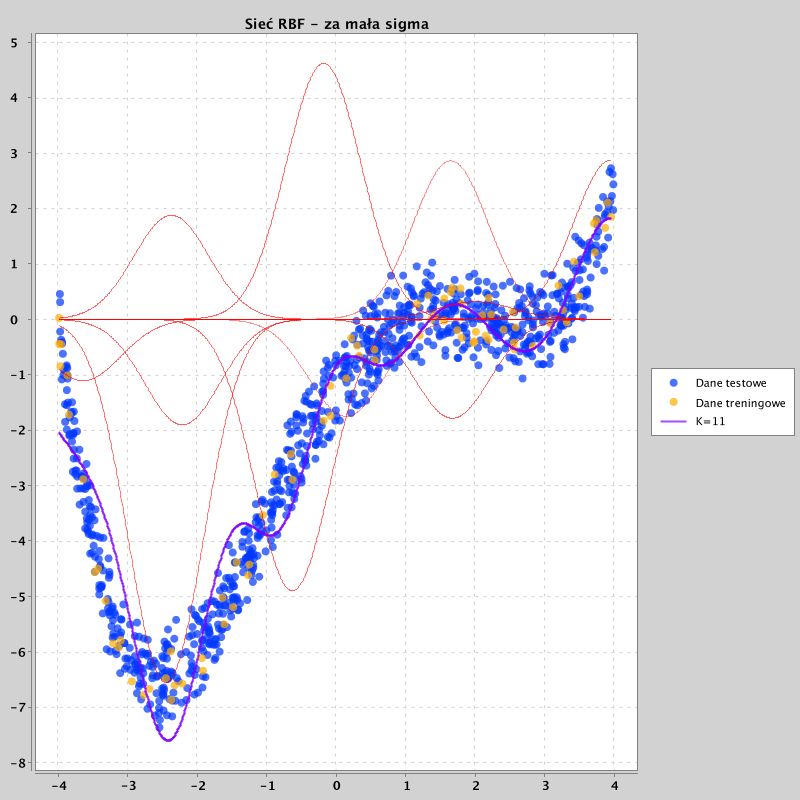
\includegraphics[width=1\linewidth]{../data/approximation3/2/small.png}
    \caption{\label{fig:2small}Za mała sigma}
  \end{minipage}
  \begin{minipage}{0.33\textwidth}
    \centering
    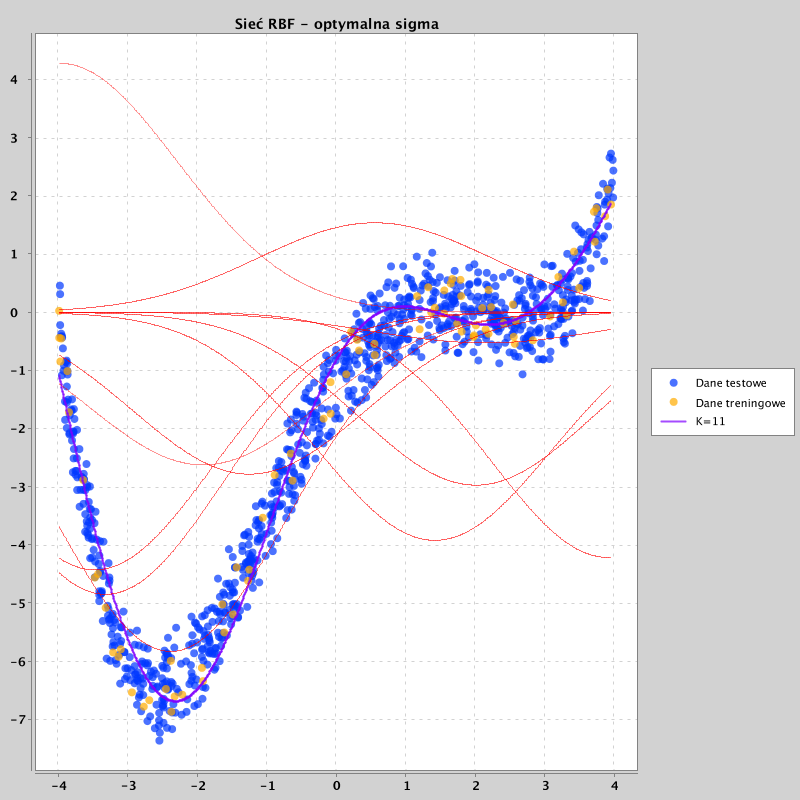
\includegraphics[width=1\linewidth]{../data/approximation3/2/optimal.png}
    \caption{\label{fig:2optimal}Optymalna sigma}
  \end{minipage}
  \begin{minipage}{0.33\textwidth}
    \centering
    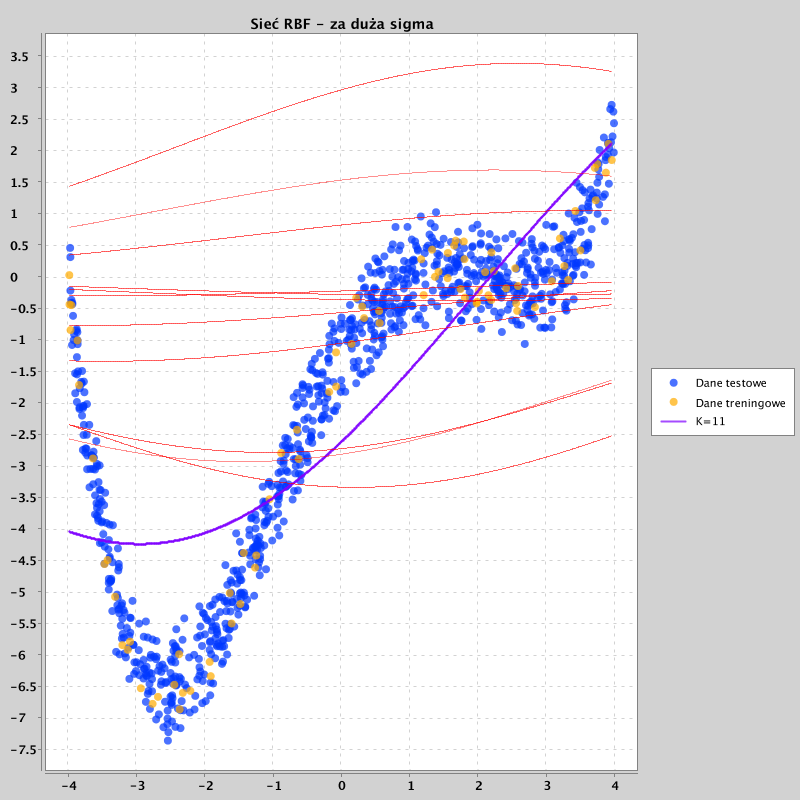
\includegraphics[width=1\linewidth]{../data/approximation3/2/big.png}
    \caption{\label{fig:2big}Za duża sigma}
  \end{minipage}\hfill
\end{figure}
Na podstawie poprzednich wyników wybrano $K=11$. Na Rysunku \ref{fig:2small} widać powód zakłóceń wykrytych na Rysunku \ref{fig:1small}.
Gdy sigma jest za mała funkcje aktywacji neuronów mają zbyt wąski obszar aktywacji.
Z drugiej strony na Rysunku \ref{fig:2big} widać, że przy dużym współczynniku skalującym funkcje neuronów są prawie stałe.
Nie da się stworzyć z kombinacji funkcji stałych dowolnej funkcji.
Jeśli zaś dobierzemy sigmę optymalnie, neurony będą realizowały funkcje nie za wąską i nie ze szeroką, co umożliwi bardzo dokładną aproksymację jak na Rysunku \ref{fig:2optimal}.


\subsection{Podzadanie 3}
Symbole $\epsilon_a$, $\epsilon_b$ oznaczają błędy średniokwadratowe odpowiednio dla zbioru treningowego i testowego. 
Symbol $\sigma$ w Tabeli \ref{table:approx3} oznacza odchylenie standardowe.
\begin{table}[h!]
  \caption{\label{table:approx3}Błąd średniokwadratowy oraz odchylenie dla zbioru treningowego i testowego dla 100 prób nauki}
  \centering
  \begin{tabular}{|l|n{1}{3}|n{1}{3}|n{1}{3}|n{1}{3}|}
    \hline
    \textbf{K} & \textbf{$avg(\epsilon_a)$} & \textbf{$\sigma(\epsilon_a)$} & \textbf{$avg(\epsilon_b)$} & \textbf{$\sigma(\epsilon_b)$}\\
    \hline
    1 & 2.2487527537653222 & 0.6261100919193574 & 1.955473836265807 & 0.5621825986540743 \\
    6 & 0.28568563944924996 & 0.2858213621279681 & 0.2522575453670399 & 0.19566409363294007 \\
    11 & 0.15128659994761162 & 0.11688975023198557 & 0.1680474127628648 & 0.07502859293396406 \\
    16 & 0.07765026065094292 & 0.02498215607290317 & 0.11514668896463105 & 0.01780284915773643 \\
    21 & 0.06057939963788164 & 0.016323733595582136 & 0.10661257959927159 & 0.009578394200630884 \\
    26 & 0.05789604352158822 & 0.009466525235758683 & 0.10751656209053062 & 0.007975489839156847 \\
    31 & 0.0515018661618608 & 0.005740971340396712 & 0.10206851520703669 & 0.005089507447365943 \\
    36 & 0.04704336994595712 & 0.0033461785075818125 & 0.09778242471482931 & 0.0032371893229406067 \\
    41 & 0.04561073842684816 & 0.0031295651169926855 & 0.09715678881154301 & 0.003091645909513203 \\
    \hline
  \end{tabular}
\end{table}
Losowy wybór centrów neuronów wprowadza dodatkowy błąd do sieci, 
gdyż przy małej ich liczbie mogą one zostać rozłożone nierównomiernie po całym zbiorze.
Wynika stąd bardzo duże odchylenie standardowe dla $K=1,6,11$.
Gdy $K=11$, błąd jest już relatywnie mały jednak nauka jest niestabilna, przez wspomniane losowanie centrów.
Zauważmy, że dla $K=16$, błąd zmniejsza się już dwukrotnie, a odchylenie standardowe jest bardzo małe.
Taka liczba neuronów zapewnia już reprezentatywność danych treningowych.
Przy $K=26,31,36,41$ średni błąd i odchylenie zmienia się nieznacząco w stosunku do $K=16$.
Za duża liczba neuronów nie zwiększa znacząco możliwości aproksymacyjnych sieci.
Błąd i odchylenie na zbiorze testowym zawsze jest większe niż na zbiorze treningowym.

\subsection{Podzadanie 4}
\begin{figure}[!htb]
  \centering
  \begin{minipage}{0.5\textwidth}
    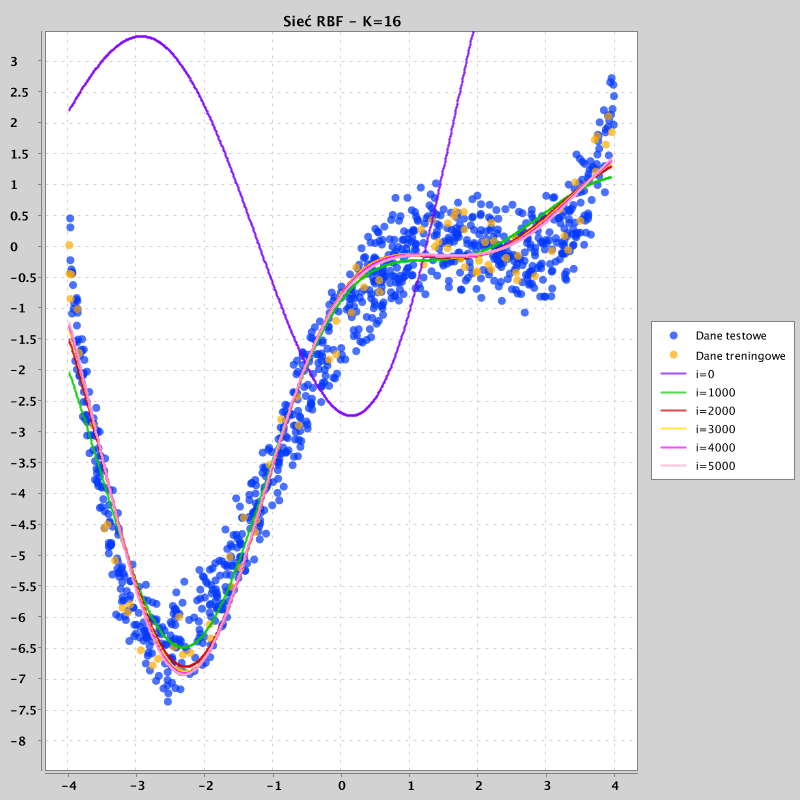
\includegraphics[width=1\linewidth]{../data/approximation3/4/chart.png}
    \caption{\label{fig:4chart}Zmiana funkcji sieci w różnych momentach}
  \end{minipage}\hfill
\end{figure}

Na podstawie obserwacji z Tabeli \ref{table:approx3},
Rysunek \ref{fig:4chart} został wygenerowany z parametrami $K=16$, liczba iteracji $= 5000$.
Można na nim wyraźnie zaobserwować, że już po $2000$ iteracji funkcja realizowana przez sieć wyglądała tak samo jak dla $i=5000$.
Gdy błąd przestanie się znacząco zmniejszać należy przestać uczyć sieć, gdyż nie da to lepszych efektów.

\subsection{Podsumowanie}
\begin{itemize}
  \item Błąd średniokwadratowy z każdą iteracją spada dosyć szybko, jednak w pewnym momencie osiąga próg, po którym dalsze uczenie sieci nie daje znaczących efektów.
  \item Potrzebna liczba neuronów w warstwie radialnej jest zależna od charakterystyki danych jakie aproksymujemy. Za mała nie przybliży jej wcale, a za duża daje prawie takie same wyniki jak optymalna, którą należy dobrać eksperymentalnie.
  \item Sieć można uznać za nauczoną, gdy jej błąd przestanie znacząco maleć. Zależy to od charakterystyki danych. Jest to dosyć ważny aspekt, gdyż wtedy można trenować sieć np. przy 5000 iteracjach, a nie 20000 iteracji, co zabiera czas i moc obliczeniową.
  \item Jeśli centra zostaną źle wylosowane to błąd znacząco się zwiększa, dlatego należy wybierać taką ich liczbe aby minimalizować błąd stworzony przez losowanie.
  \item Współczynnik skalujący ma ogromny wpływ na funkcje realizowaną przez sieć, gdy dobierzemy go źle to przy za małej wartości sieć będzie niedokładna. Przy za dużym współczynniku nie będzie aproksymowała wcale. Należy go dobierać tak, aby był optymalny.
\end{itemize}

\section{Osobna nauka warstw - klasyfikacja}
Wykorzystano parametry nauki: $\alpha=0.05$, optymalna sigma, liczba iteracji $=5000$.
Centra dobierano za pomocą algorytmu K-Średnich.
\subsection{Podzadanie 1}
\begin{figure}[!htb]
  \begin{minipage}{0.33\textwidth}
    \centering
    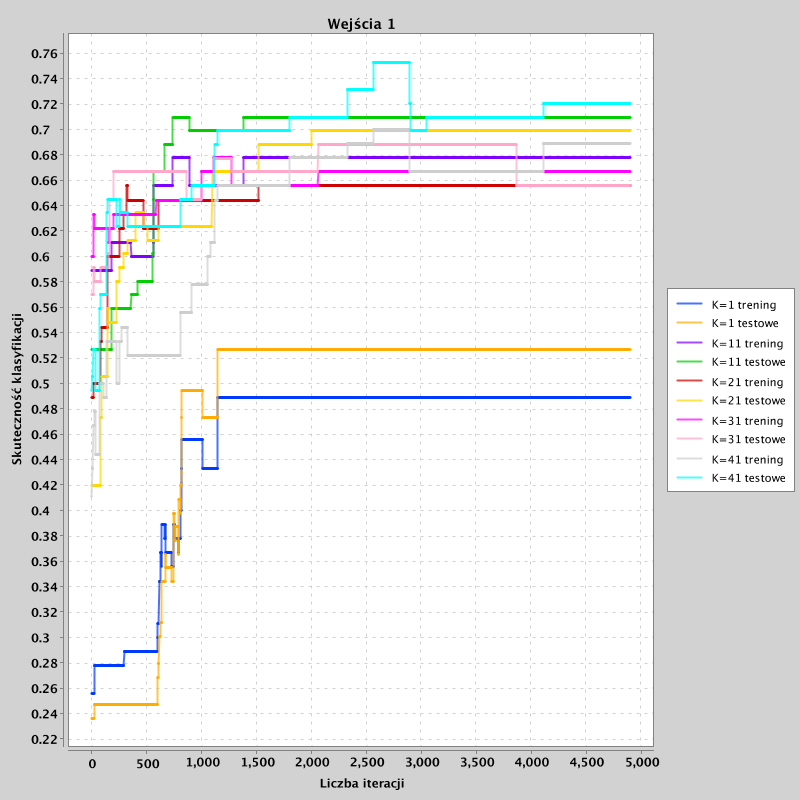
\includegraphics[width=1\linewidth]{../data/classification4/1/1_1.png}
    \caption{\label{fig:41_1_1}}
  \end{minipage}
  \begin{minipage}{0.33\textwidth}
    \centering
    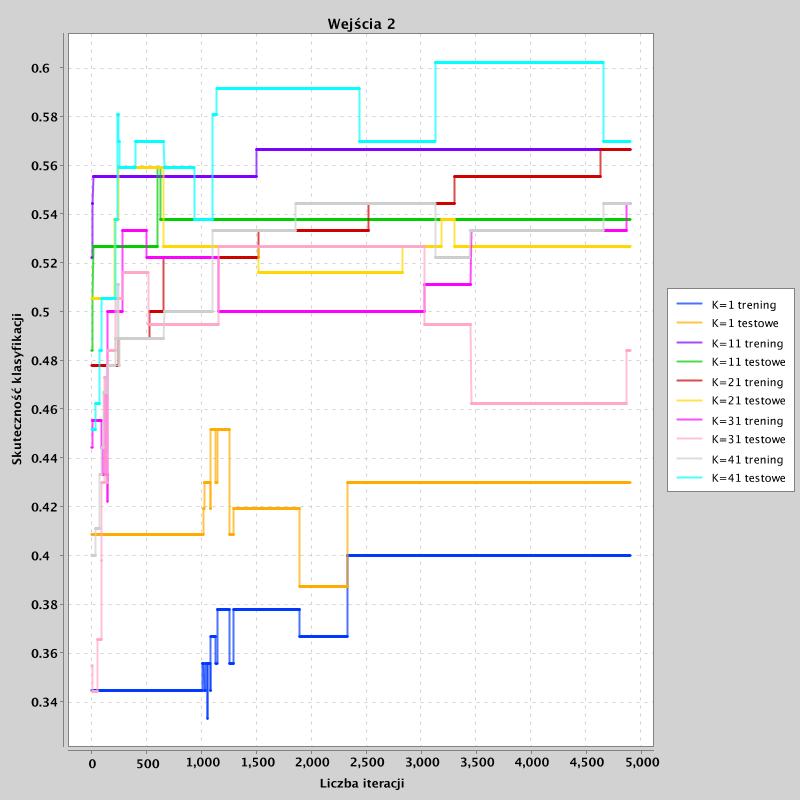
\includegraphics[width=1\linewidth]{../data/classification4/1/1_2.png}
    \caption{\label{fig:41_1_2}}
  \end{minipage}
  \begin{minipage}{0.33\textwidth}
    \centering
    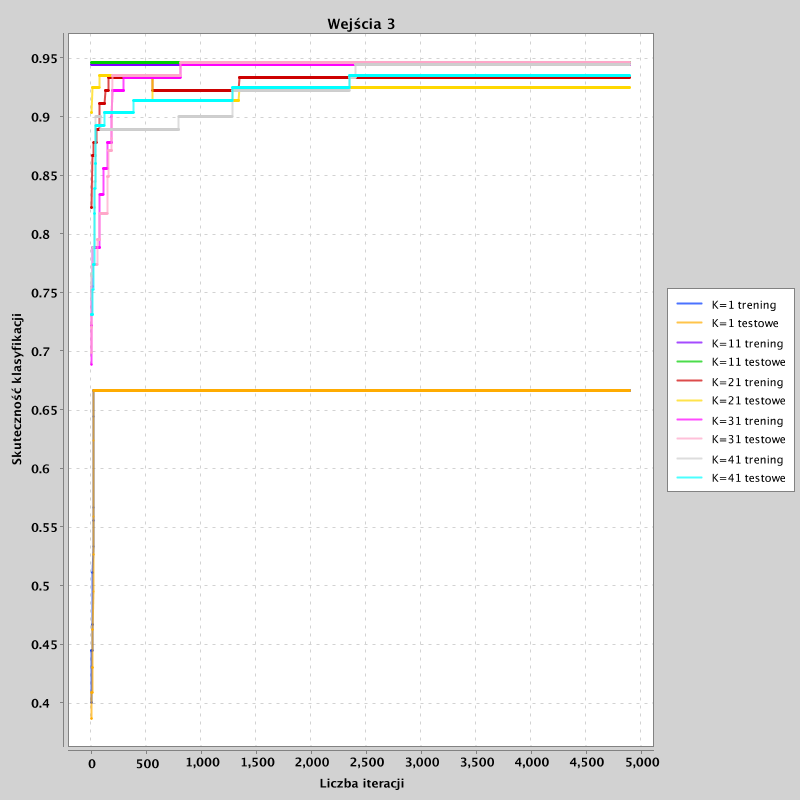
\includegraphics[width=1\linewidth]{../data/classification4/1/1_3.png}
    \caption{\label{fig:41_1_3}}
  \end{minipage}\hfill
\end{figure}
\begin{figure}[!htb]
  \begin{minipage}{0.33\textwidth}
    \centering
    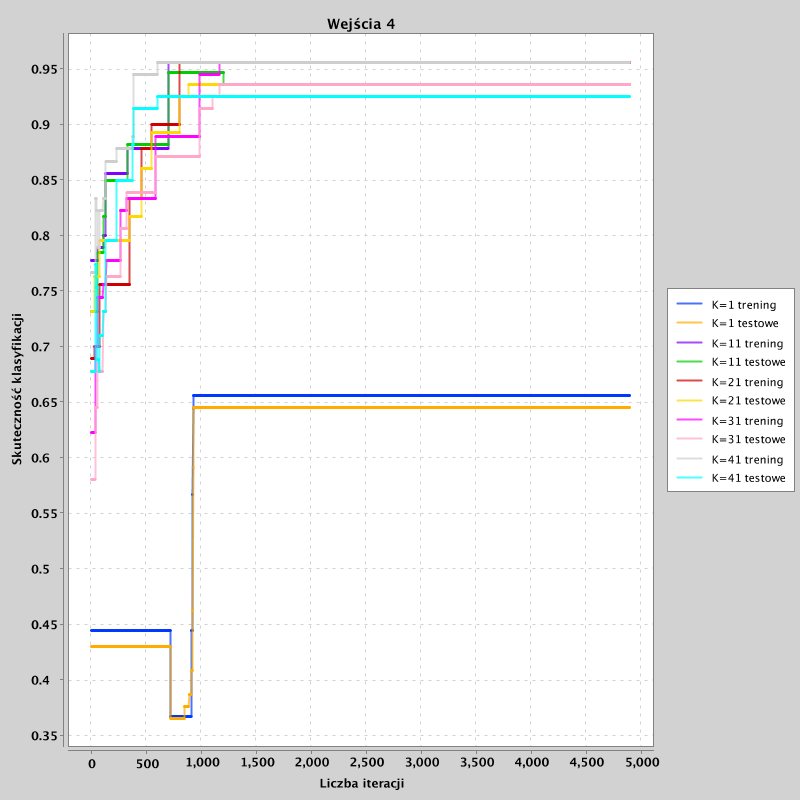
\includegraphics[width=1\linewidth]{../data/classification4/1/1_4.png}
    \caption{\label{fig:41_1_4}}
  \end{minipage}
  \begin{minipage}{0.33\textwidth}
    \centering
    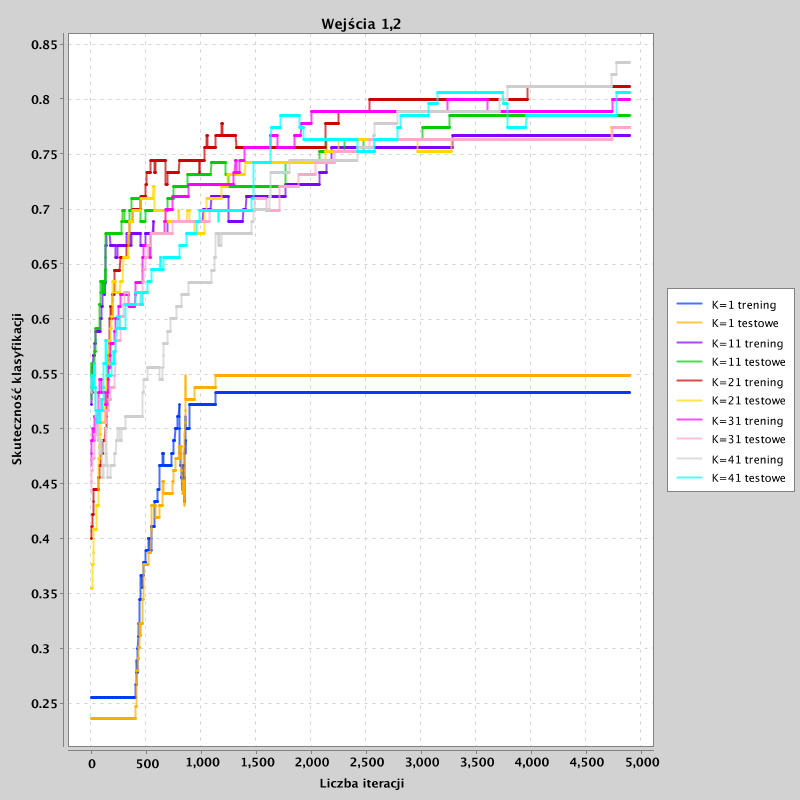
\includegraphics[width=1\linewidth]{../data/classification4/1/2_1,2.png}
    \caption{\label{fig:41_2_1,2}}
  \end{minipage}
  \begin{minipage}{0.33\textwidth}
    \centering
    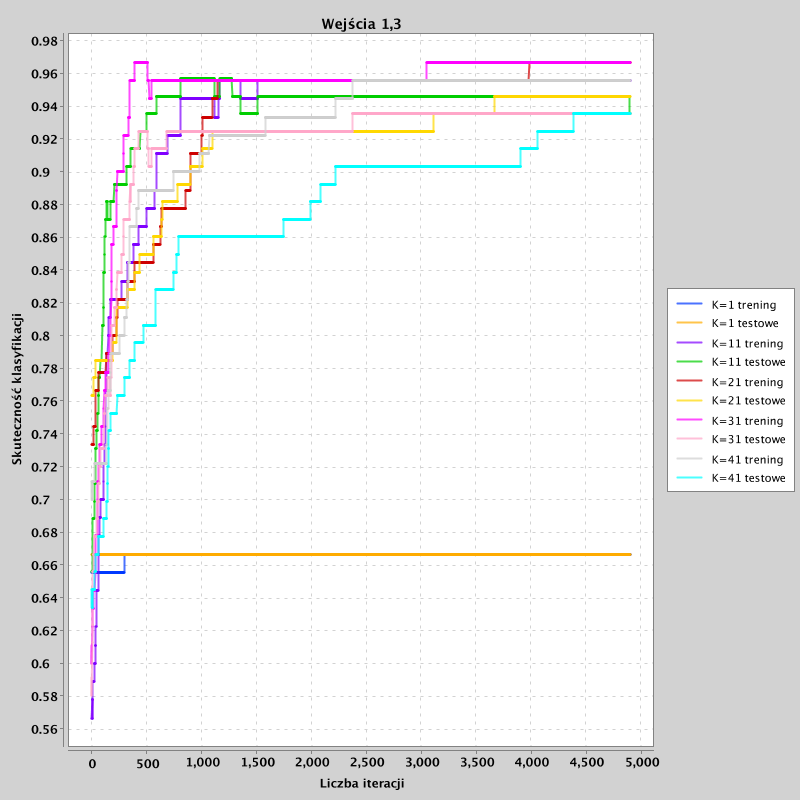
\includegraphics[width=1\linewidth]{../data/classification4/1/2_1,3.png}
    \caption{\label{fig:41_2_1,3}}
  \end{minipage}\hfill
\end{figure}
\begin{figure}[!htb]
  \begin{minipage}{0.33\textwidth}
    \centering
    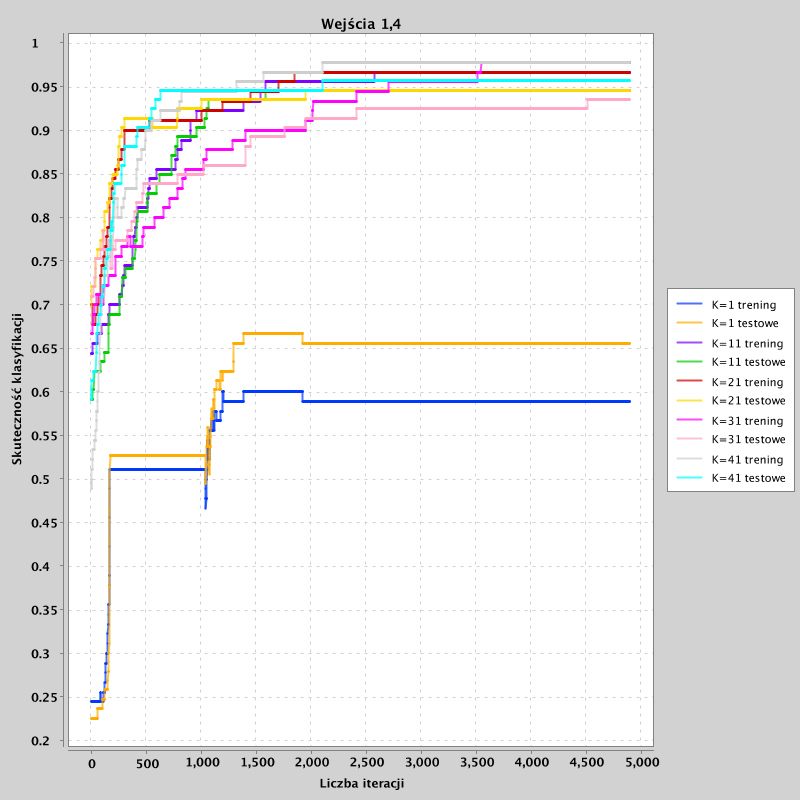
\includegraphics[width=1\linewidth]{../data/classification4/1/2_1,4.png}
    \caption{\label{fig:41_2_1,4}}
  \end{minipage}
  \begin{minipage}{0.33\textwidth}
    \centering
    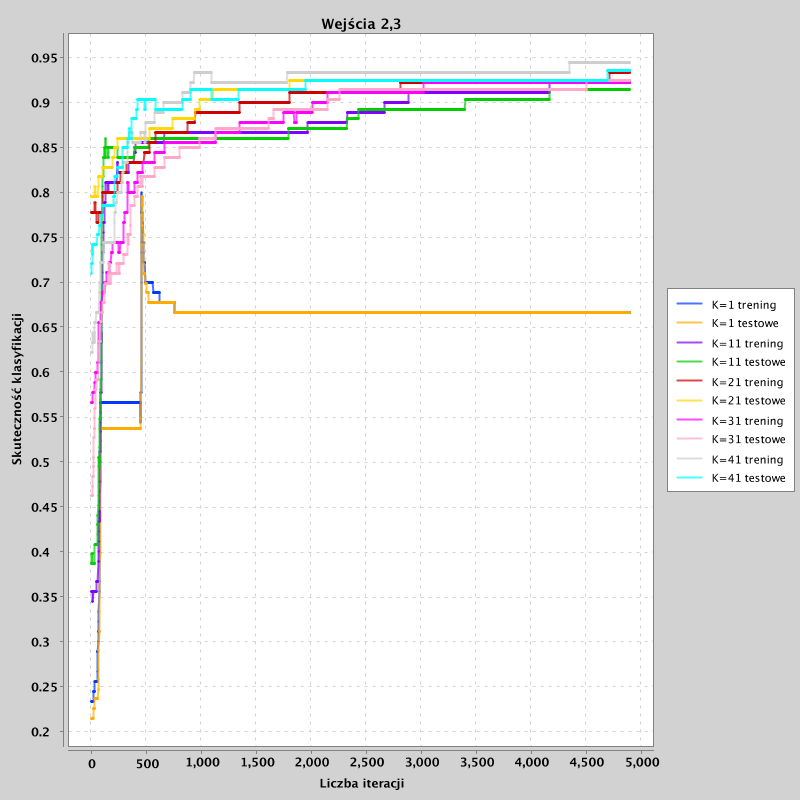
\includegraphics[width=1\linewidth]{../data/classification4/1/2_2,3.png}
    \caption{\label{fig:41_2_2,3}}
  \end{minipage}
  \begin{minipage}{0.33\textwidth}
    \centering
    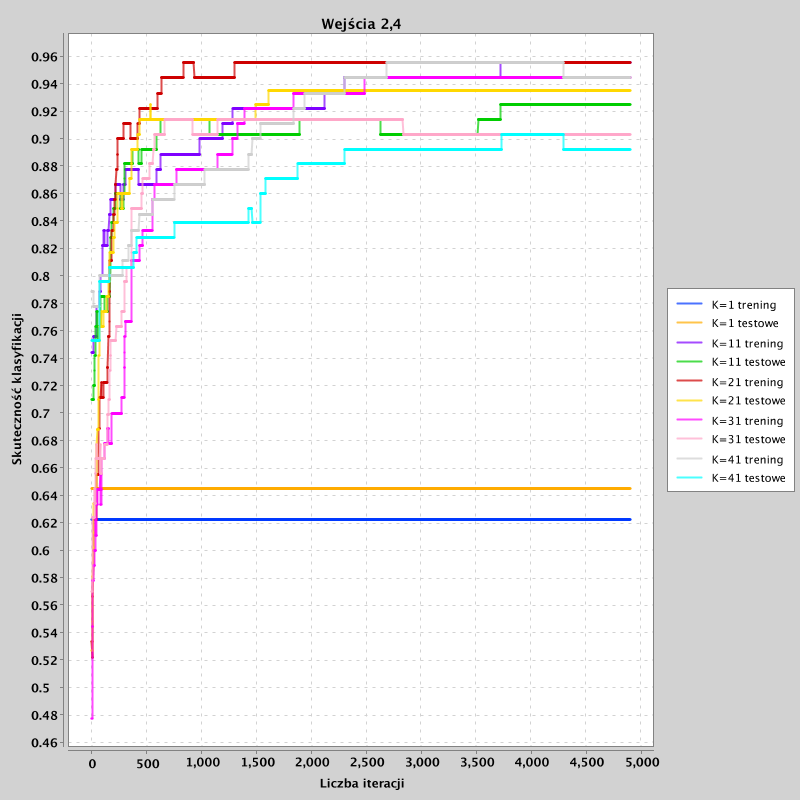
\includegraphics[width=1\linewidth]{../data/classification4/1/2_2,4.png}
    \caption{\label{fig:41_2_2,4}}
  \end{minipage}\hfill
\end{figure}
\begin{figure}[!htb]
  \begin{minipage}{0.33\textwidth}
    \centering
    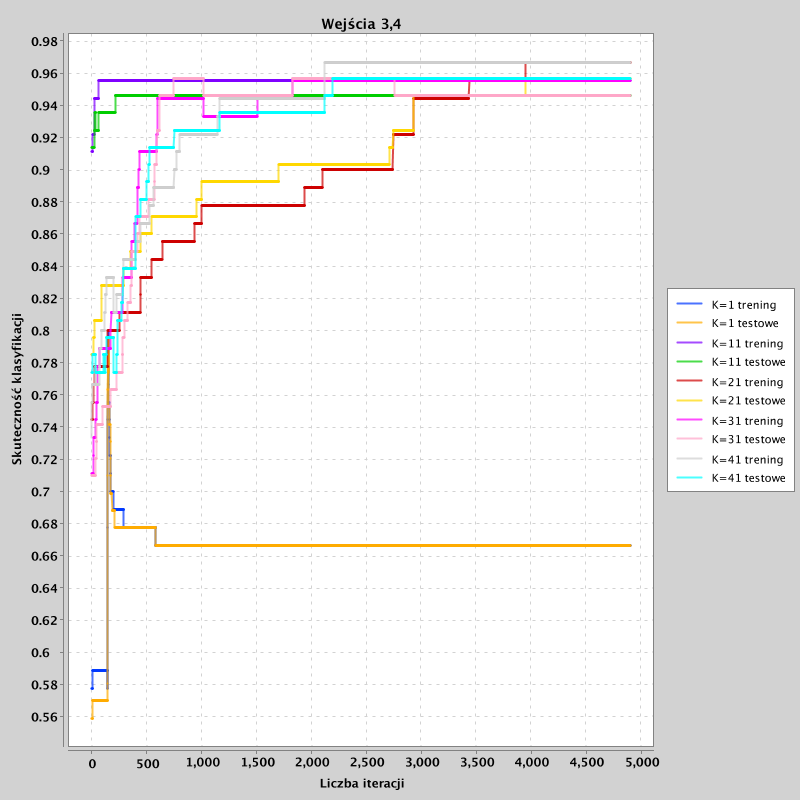
\includegraphics[width=1\linewidth]{../data/classification4/1/2_3,4.png}
    \caption{\label{fig:41_2_2,3}}
  \end{minipage}
  \begin{minipage}{0.33\textwidth}
    \centering
    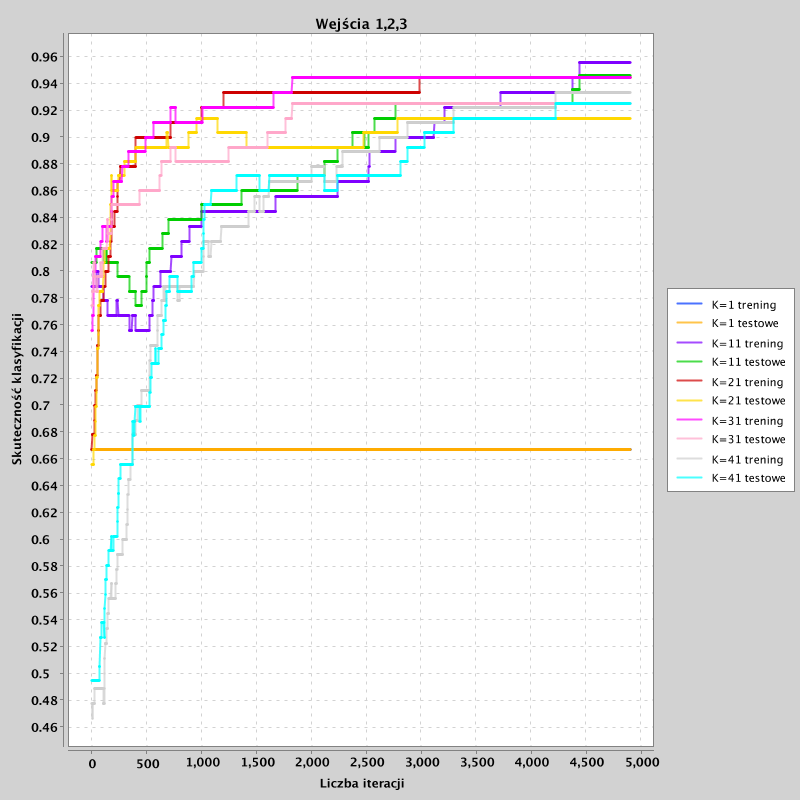
\includegraphics[width=1\linewidth]{../data/classification4/1/3_1,2,3.png}
    \caption{\label{fig:41_3_1,2,3}}
  \end{minipage}
  \begin{minipage}{0.33\textwidth}
    \centering
    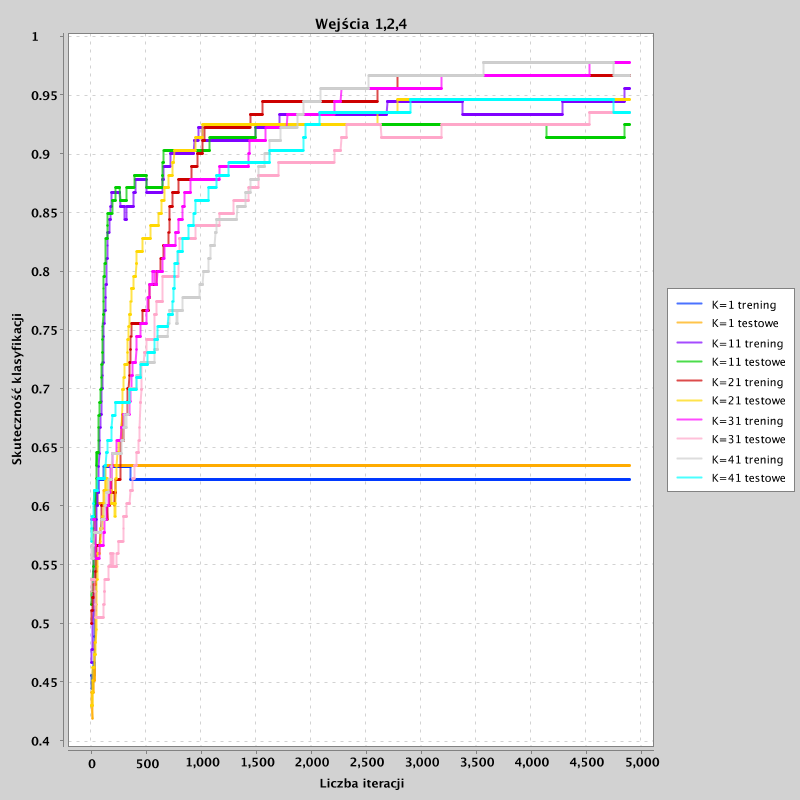
\includegraphics[width=1\linewidth]{../data/classification4/1/3_1,2,4.png}
    \caption{\label{fig:41_3_1,2,4}}
  \end{minipage}\hfill
\end{figure}
\begin{figure}[!htb]
  \begin{minipage}{0.33\textwidth}
    \centering
    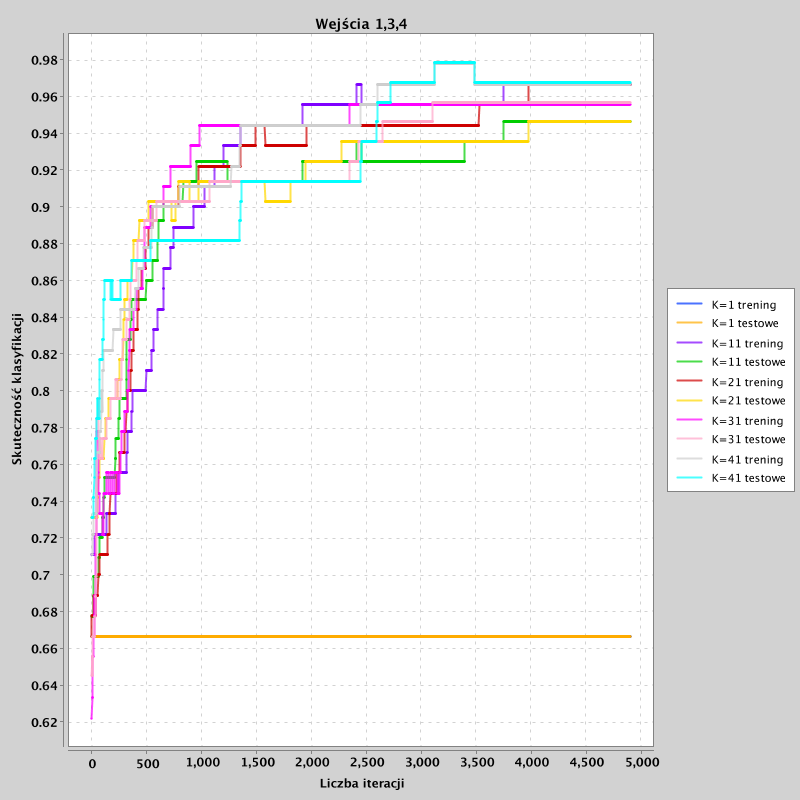
\includegraphics[width=1\linewidth]{../data/classification4/1/3_1,3,4.png}
    \caption{\label{fig:41_3_1,3,4}}
  \end{minipage}
  \begin{minipage}{0.33\textwidth}
    \centering
    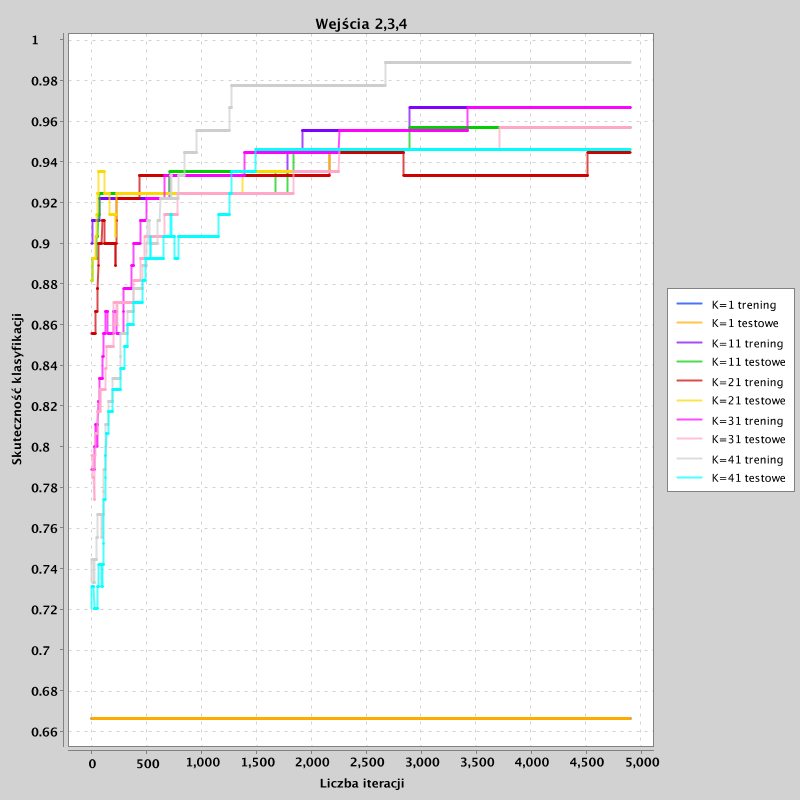
\includegraphics[width=1\linewidth]{../data/classification4/1/3_2,3,4.png}
    \caption{\label{fig:41_3_2,3,4}}
  \end{minipage}
  \begin{minipage}{0.33\textwidth}
    \centering
    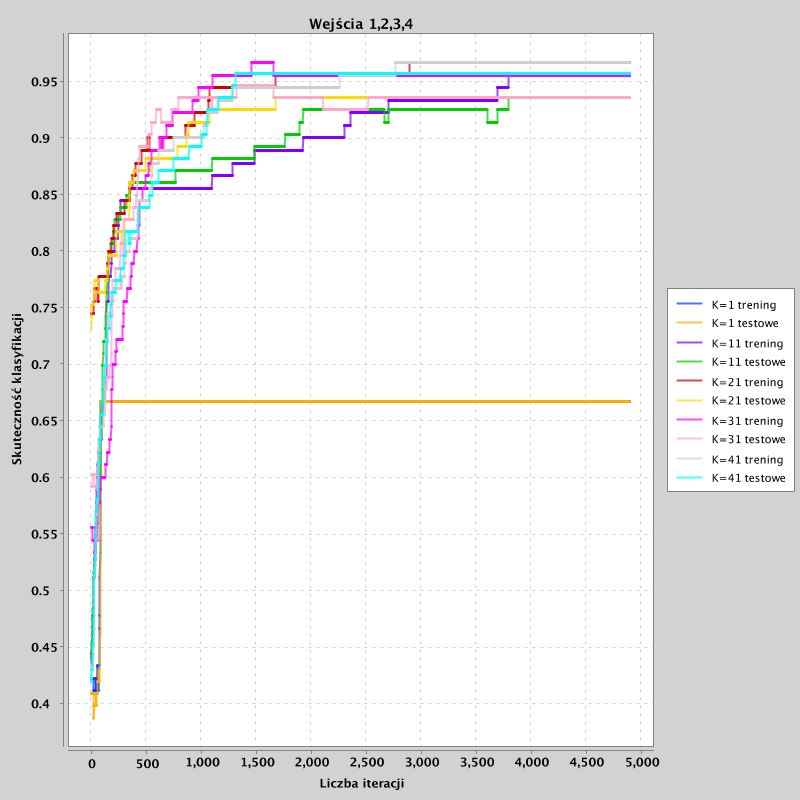
\includegraphics[width=1\linewidth]{../data/classification4/1/4_1,2,3,4.png}
    \caption{\label{fig:41_4_1,2,3,4}}
  \end{minipage}\hfill
\end{figure}

\nprounddigits{2}
\subsection{Podzadanie 2}
W Tabeli \ref{table:classify4} $p_a$, $p_b$ oznaczają odpowiednio procent klasyfikacji dla zbioru treningowego i testowego.
\begin{table}[h!]
  \caption{\label{table:classify4}Procent klasyfikacji oraz odchylenie dla zbioru treningowego i testowego dla 100 prób nauki}
  \centering
  \begin{tabular}{|l|n{1}{3}|n{1}{3}|n{1}{3}|n{1}{3}|}
    \hline
    \textbf{K} & \textbf{$avg(p_a)$} & \textbf{$\sigma(p_a)$} & \textbf{$avg(p_b)$} & \textbf{$\sigma(p_b)$} \\
    \hline
    1 & 0.6666666666666659 & 0 & 0.6666666666666659 & 0 \\
    6 & 0.935111111111111 & 0.0053794304164045135 & 0.928494623655913 & 0.009542064166289733 \\
    11 & 0.9368888888888887 & 0.005183068350973578 & 0.9307526881720424 & 0.01057049955048994 \\
    16 & 0.9371111111111108 & 0.006130272988503856 & 0.9308602150537629 & 0.01056338744688961 \\
    21 & 0.9378888888888883 & 0.006866450913546816 & 0.9324731182795698 & 0.01043398664146946 \\
    26 & 0.9398888888888883 & 0.0056862407030773094 & 0.9349462365591399 & 0.010129808430869264 \\
    31 & 0.9422222222222213 & 0.004444444444444427 & 0.9375268817204311 & 0.010051894484440608 \\
    36 & 0.9423333333333324 & 0.004358898943540653 & 0.9377419354838716 & 0.010676612602035777 \\
    41 & 0.9429999999999988 & 0.004622809791714378 & 0.9398924731182804 & 0.010869792434046578 \\
    \hline
  \end{tabular}
\end{table}

\subsection{Podzadanie 3}
\begin{figure}[!htb]
  \begin{minipage}{0.33\textwidth}
    \centering
    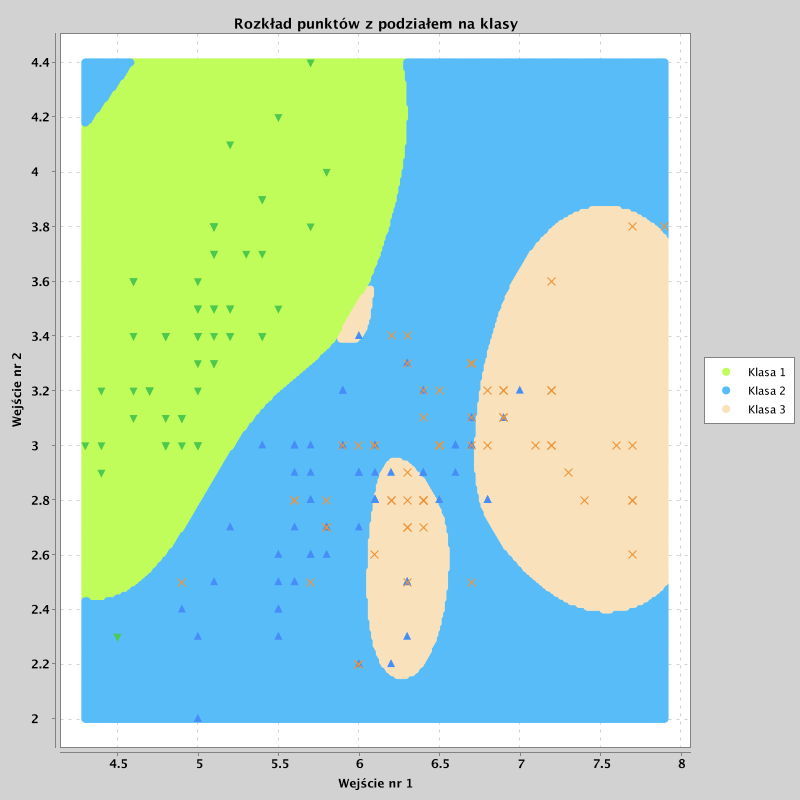
\includegraphics[width=1\linewidth]{../data/classification4/3/2_1,2.png}
    \caption{\label{fig:42_2_1,2}}
  \end{minipage}
  \begin{minipage}{0.33\textwidth}
    \centering
    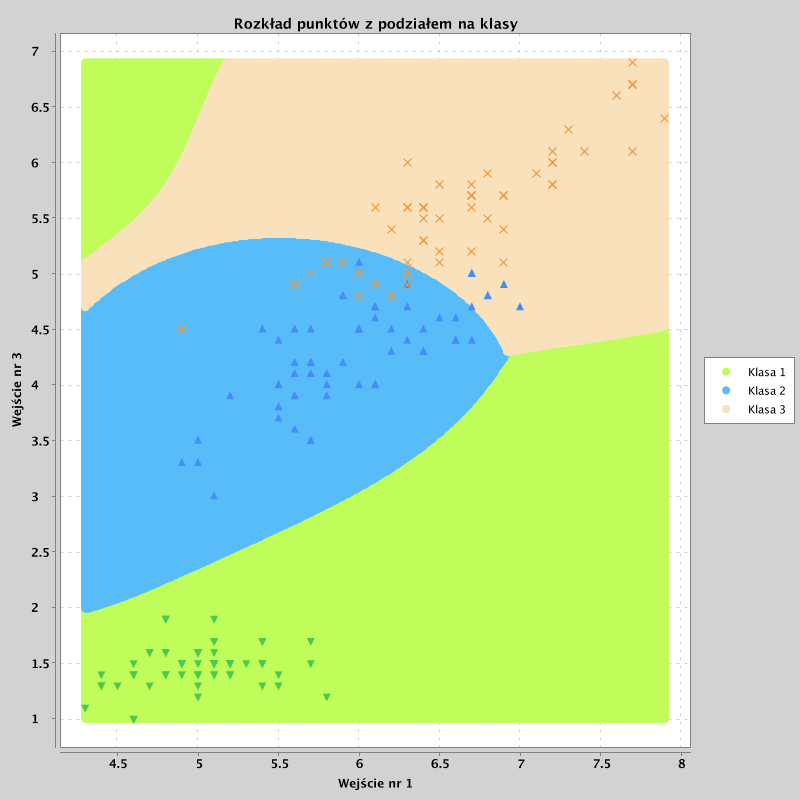
\includegraphics[width=1\linewidth]{../data/classification4/3/2_1,3.png}
    \caption{\label{fig:42_2_1,3}}
  \end{minipage}
  \begin{minipage}{0.33\textwidth}
    \centering
    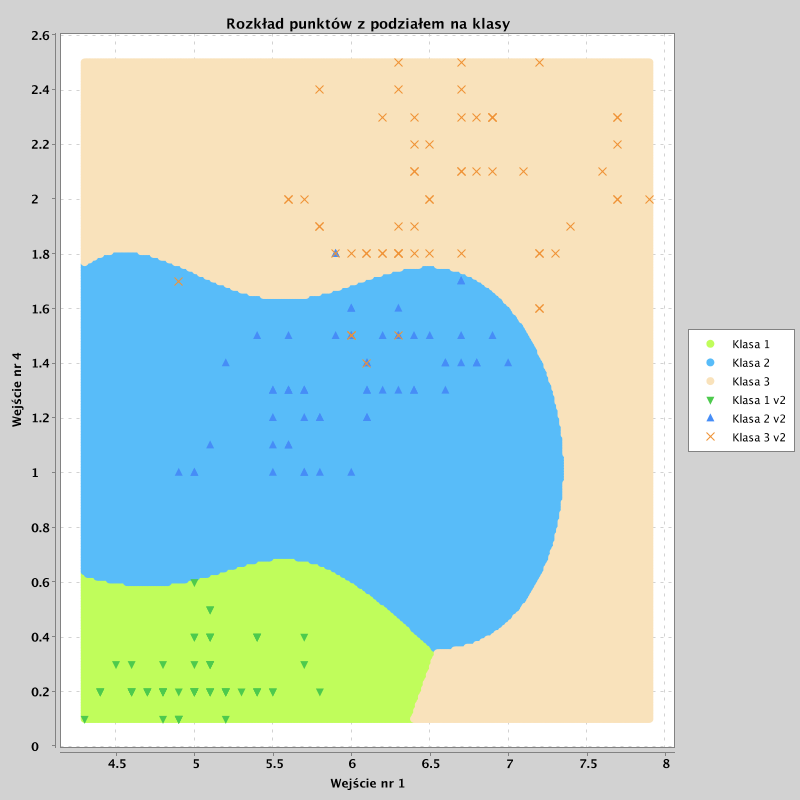
\includegraphics[width=1\linewidth]{../data/classification4/3/2_1,4.png}
    \caption{\label{fig:42_2_1,4}}
  \end{minipage}\hfill
\end{figure}
\begin{figure}[!htb]
  \begin{minipage}{0.33\textwidth}
    \centering
    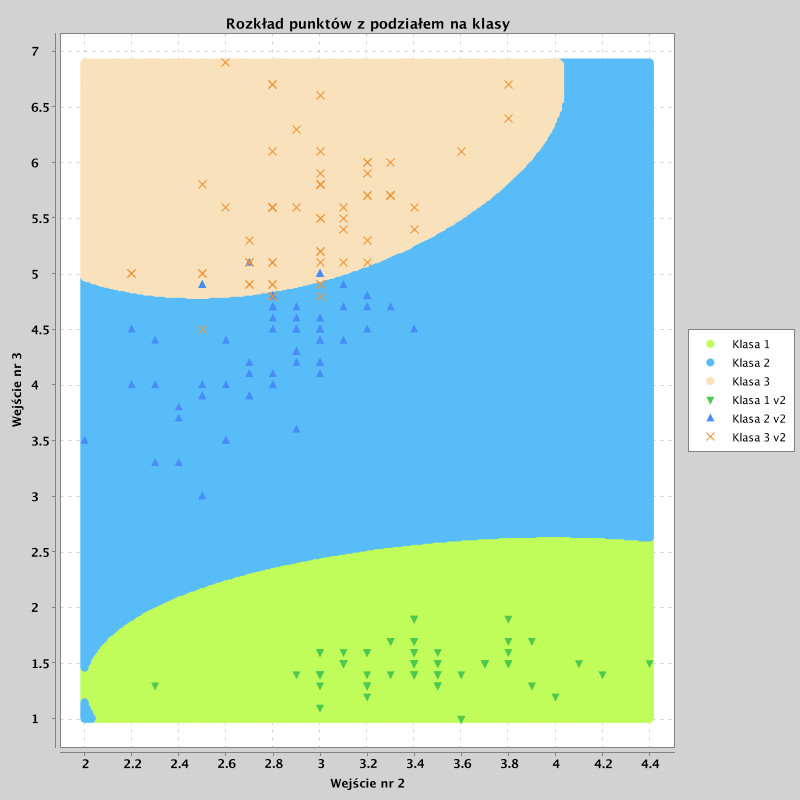
\includegraphics[width=1\linewidth]{../data/classification4/3/2_2,3.png}
    \caption{\label{fig:42_2_2,3}}
  \end{minipage}
  \begin{minipage}{0.33\textwidth}
    \centering
    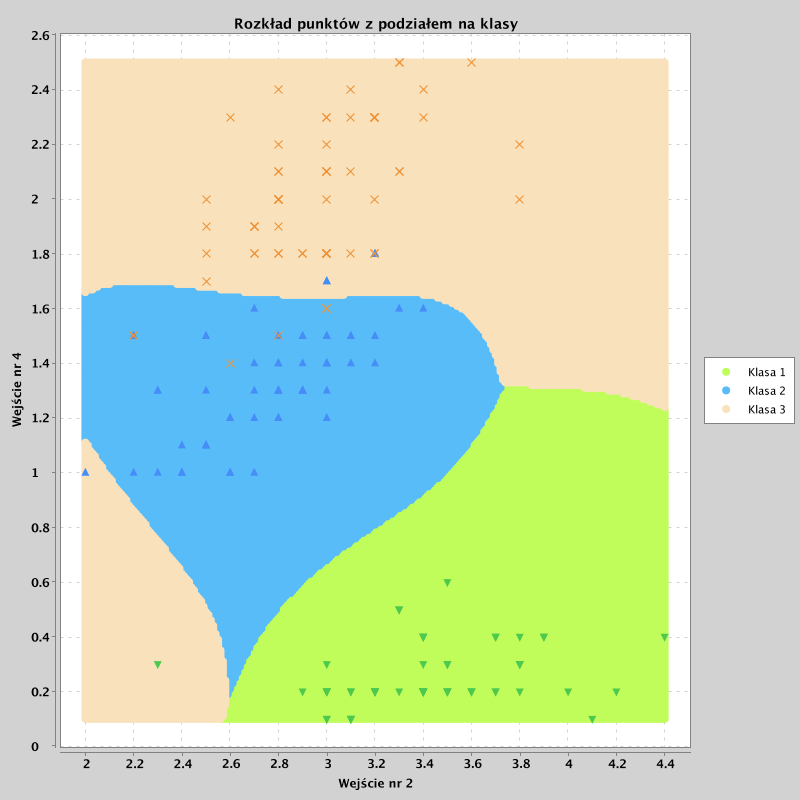
\includegraphics[width=1\linewidth]{../data/classification4/3/2_2,4.png}
    \caption{\label{fig:42_2_2,4}}
  \end{minipage}
  \begin{minipage}{0.33\textwidth}
    \centering
    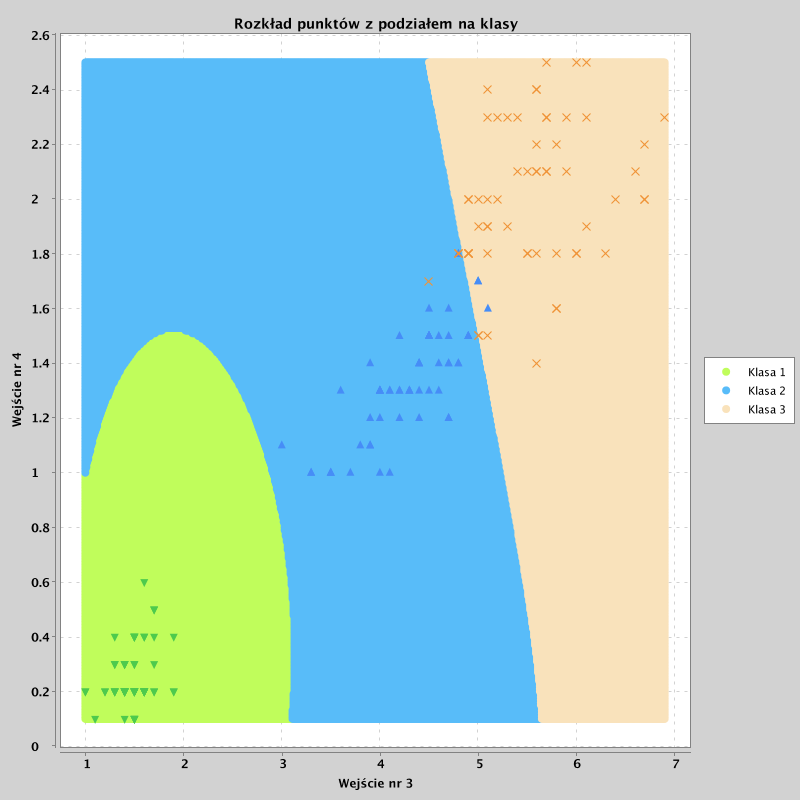
\includegraphics[width=1\linewidth]{../data/classification4/3/2_3,4.png}
    \caption{\label{fig:42_2_3,4}}
  \end{minipage}\hfill
\end{figure}


\section{Nauka obu warstw}
\newcommand{\partialSigma}{\frac{\partial}{\partial{\sigma_{k}}}}
\begin{equation}
  \partialSigma = \frac{1}{N} \sum_{j=1}^{N}  (f(x^j) - y^j) z_k(x^j) d^2(x^j, c_k) \frac{1}{\sigma_{k}^3}
\end{equation}
\subsection{Pochodna po współczynniku skalującym}
\begin{align}
  \frac{\partial E}{\partial{\sigma_{k}}}&= \frac{1}{2N} \sum_{j=1}^{N} (f(x^j) - y^j)^2\\
  &= \frac{1}{2N} \sum_{j=1}^{N} 2 (f(x^j) - y^j) f'(x^j)\\
  &= \frac{1}{N} \sum_{j=1}^{N} f(x^j - y^j) \partialSigma \sum_{k=0}^{K} w_k z_k(x^j)\\
  \partialSigma \sum_{k=0}^{K} w_k z_k(x^j) &= \sum_{k=0}^{K} w_k z_k(x^j) =  w_k \frac{\partial}{\partial{\sigma_{k}}}z_k(x^j)
\end{align}
Ponieważ tylko $w_k \partialSigma z_k(x^j)$ zależy od $\sigma_k$, dla $k=0, ..., K$
\begin{align}
  \frac{\partial}{\partial{\sigma_{k}}}z_k(x^j) &= \partialSigma exp(-d^2(x^j, c_k) \frac{1}{2\sigma_k^2})\\
  &= z_k(x^j) \partialSigma ( \frac{1}{2\sigma_k^2}) \\
  &= z_k(x^j) \frac{-1}{2} d^2(x^j, c_k) \partialSigma {\sigma_k^{-2}}\\
  &= z_k(x^j) \frac{-1}{2} d^2(x^j, c_k) -2 \sigma_k^{-3}\\
  &= z_k(x^j) d^2(x^j, c_k) \frac{1}{\sigma_k^3}
\end{align}
Ostatecznie
\begin{equation}
  \frac{\partial E}{\partial{\sigma_{k}}} = \frac{1}{N} \sum_{j=1}^{N} f(x^j - y^j) z_k(x^j) w_k d^2(x^j, c_k) \frac{1}{\sigma_k^3}
\end{equation}
\subsection{Pochodna po koordynacie centrum neuronu}
\begin{align}
  \frac{\partial E}{\partial{c_{k,i}}} &= \frac{1}{2N} \sum_{j=1}^{N} (f(x^j) - y^j)^2\\
  &= \frac{1}{2N} \sum_{j=1}^{N} 2 f(x^j - y^j) f'(x^j)\\
  &= \frac{1}{N} \sum_{j=1}^{N} f(x^j - y^j) \frac{\partial}{\partial{c_{k,i}}} \sum_{k=0}^{K} w_k z_k(x^j)
\end{align}
\begin{equation}
  \frac{\partial}{\partial{c_{k,i}}} \sum_{k=0}^{K} w_k z_k(x^j) = \sum_{k=0}^{K} w_k z_k(x^j) =  w_k \frac{\partial}{\partial{c_{k,i}}}z_k(x^j)
\end{equation}
Ponieważ tylko $w_k \frac{\partial}{\partial{c_{k,i}}}z_k(x^j)$ zależy od $c_{k,i}$, dla $k=1, ..., K$
\begin{align}
  w_k \frac{\partial}{\partial{c_{k,i}}}z_k(x^j) &= w_k \frac{\partial}{\partial{c_{k,i}}} exp(-d^2(x^j, c_k) \frac{1}{2\sigma_k^2})\\
    &= w_k z_k(x^j) \frac{\partial}{\partial{c_{k,i}}} -d^2(x^j, c_k) \frac{1}{2\sigma_k^2}\\
    &= w_k z_k(x^j) \frac{-1}{2\sigma_k^2} \frac{\partial}{\partial{c_{k,i}}} d^2(x^j, c_k) \\
  \frac{\partial}{\partial{c_{k,i}}} d^2(x^j, c_k) &= \frac{\partial}{\partial{c_{k,i}}} \sqrt{\sum_{i = 1}^{n} (x_i - c_{k,i})^2}^2\\
  &= \frac{\partial}{\partial{c_{k,i}}} \sum_{i = 1}^{n} (x_i - c_{k,i})^2\\
  &= \sum_{i = 1}^{n} 2 (x_i - c_{k,i}) (-1)\\
  &= -2 \sum_{i = 1}^{n} (x_i - c_{k,i})\\
  &= -2 (x_i - c_{k,i})
\end{align}
Ponieważ tylko $x_i - c_{k,i}$ zależy od $c_{k,i}$.
\begin{align}
  w_k z_k'(x^j) &= w_k z_k(x^j) \frac{-1}{2\sigma_k^2} -2 (x_i - c_{k,i})\\
  w_k z_k'(x^j) &= w_k z_k(x^j) \frac{1}{\sigma_k^2} (x_i - c_{k,i})\\
\end{align}
Ostateczny wzór:
\begin{equation}
\frac{\partial E}{\partial{c_{k,i}}} = \frac{1}{N} \sum_{j=1}^{N} f(x^j - y^j) w_k z_k(x^j) \frac{1}{\sigma_k^2} (x_i - c_{k,i})
\end{equation}

\end{document}